\documentclass[tikz,border=2pt]{standalone}
\usepackage{amsmath}
\usepackage{pgfplots}
\pgfplotsset{compat=1.18}
\usetikzlibrary{arrows.meta}
\begin{document}
% x_{t+2} - x_{t+1} + x_t = 0: p(r) = r^2 - r + 1 has the roots e^{+-i pi/3} on the unit circle
% (left); the solution with x_0 = x_1 = 1 is 1, 1, 0, -1, -1, 0, 1, ... with period 6 (right).
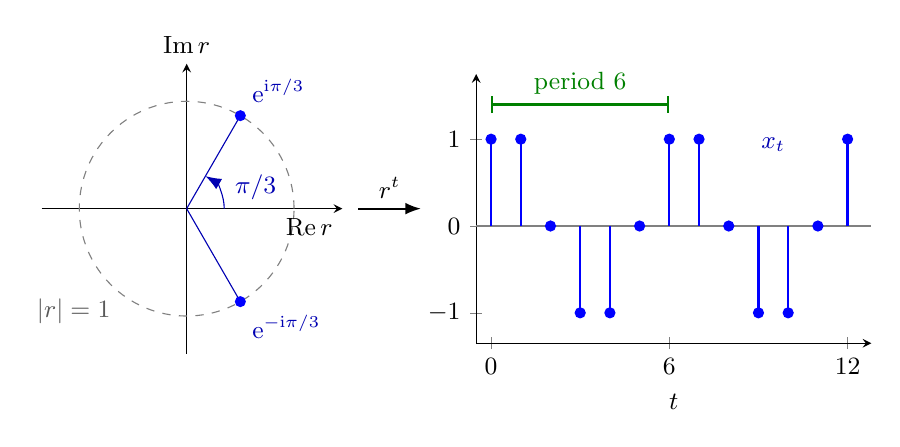
\begin{tikzpicture}[font=\small, >={Latex[length=2mm]}]
  \begin{axis}[
    name=roots, axis lines=middle, width=5.4cm, height=5.4cm, axis equal image,
    xmin=-1.35, xmax=1.45, ymin=-1.35, ymax=1.35,
    xtick=\empty, ytick=\empty, xlabel={$\operatorname{Re} r$}, ylabel={$\operatorname{Im} r$},
    xlabel style={anchor=north east}, ylabel style={anchor=south},
    clip=false
    ]
    \draw[gray, thin, dashed] (axis cs:0,0) circle[radius=1];
    \draw[blue!70!black, thin] (axis cs:0,0) -- (axis cs:0.5,0.866);
    \draw[blue!70!black, thin] (axis cs:0,0) -- (axis cs:0.5,-0.866);
    \draw[->, blue!70!black, thin] (axis cs:0.35,0) arc[start angle=0, end angle=60, radius=0.35];
    \node[blue!70!black, anchor=west] at (axis cs:0.36,0.2) {$\pi/3$};
    \node[gray!70!black, anchor=north east] at (axis cs:-0.62,-0.75) {$|r|=1$};
    \fill[blue] (axis cs:0.5,0.866) circle (2pt);
    \fill[blue] (axis cs:0.5,-0.866) circle (2pt);
    \node[blue!70!black, anchor=south west] at (axis cs:0.52,0.9) {$\mathrm{e}^{\mathrm{i}\pi/3}$};
    \node[blue!70!black, anchor=north west] at (axis cs:0.52,-0.9) {$\mathrm{e}^{-\mathrm{i}\pi/3}$};
  \end{axis}
  \begin{axis}[
    at={(roots.east)}, anchor=west, xshift=1.7cm,
    axis lines=left, width=6.6cm, height=5.0cm,
    xmin=-0.5, xmax=12.8, ymin=-1.35, ymax=1.75, xtick={0,6,12}, ytick={-1,0,1},
    xlabel={$t$}, clip=false
    ]
    \draw[gray, thin] (axis cs:-0.5,0) -- (axis cs:12.8,0);
    \addplot[blue, thick, ycomb, mark=*, mark size=1.6pt]
      coordinates {(0,1) (1,1) (2,0) (3,-1) (4,-1) (5,0) (6,1) (7,1) (8,0) (9,-1) (10,-1) (11,0) (12,1)};
    \draw[green!50!black, thick, |-|] (axis cs:0,1.4) -- (axis cs:6,1.4)
      node[midway, above] {period $6$};
    \node[blue!70!black, anchor=south] at (axis cs:9.5,0.75) {$x_t$};
  \end{axis}
  \draw[->, thick] ([xshift=0.2cm]roots.east) -- ++(0.8,0) node[midway, above] {$r^t$};
\end{tikzpicture}
\end{document}
